\chapter{Introduction to Mean curvature flow}

We introduce the second fundamental form and mean curvature associated to an immersion of a hypersurface. The mean curvature flow is then is the negative gradient flow of the volume functional on hypersurfaces. 
\section{Fundamentals of hypersurfaces}

Let $M^{n}$ be a smooth $ n $-dimensional manifold with a smooth immersion $ X : M^{n} \to \R^{n+1} $. If $ X $ is a diffeomorphism onto its image, we say $ X $ is an \textbf{embedding}  and its image $ \mathcal{M}^{n} = X(M^{n}) $ has the structure of a smooth $ n $-dimensional submanifold of $ \R^{n+1} $. We say that $ M^{n} $ is an \textbf{immersed hypersurface} and $ \mathcal{M} $ is an \textbf{embedded hypersurface} respectively. Throughout this book we will denote the embedded manifold $ X(M) $ by script $ \mathcal{M} $ to differentiate between the domain and its image. Let $ (U, \{x^{i}\}) $ be a coordinate system on $ M^{m} $, in Euclidean coordinates the pushforward of tangent vectors will be 
    \[ dX( \partial_{i}) \define \frac{ \partial X}{ \partial x^{i}} = \partial_{i}X \]
where $ dX : TM^{n} \to T\R^{n+1} $ is the derivative of $ X $. Since $ dX $ is an injection for each point in $ M^{n} $, we can define an inner product on $ TM^{n} $ which in local coordinates is given by 
    \[ g( \partial_{i}, \partial_{j}) = \left< \partial_{i}X, \partial_{j}X \right> \]
where $ \left< \cdot, \cdot \right> $ denotes the standard inner product on Euclidean space. Further we can define the Levi-Civita connection on $ M^{n} $ from the Levi-Civita connection on $ \R^{n+1} $. Let $ X_{p} \in T_{p}\Rn $ be a vector and $ Y : U \to T\Rn|_{U} $ be a local vector field in a neighborhood $ U $ containing $ p $. The Levi-Civita connection of $ Y $ with respect to $ X $ on  $ \R^{n+1} $ is given by 
\[ D_{X_{p}}Y =  X_{p}(Y^{i}) \partial_{i}\]
where $ Y = (Y^{1}, \ldots , Y^{n+1}) $ are the components of $ Y $ in the standard coordinates. Using the immersion condition, we define a connection on $ TM^{n} $ induced from $ D $.  Let $ x \in M^{n} $ and $ u \in T_{p}M^{n}, \tilde{v} \in TM^{n}|_{U}$ for some open set $ U $ containing $ x $. Define a connection $ \nabla $ by 
\begin{equation}
    dX(\nabla_{u}\tilde{v}) = D_{dX(u)}(\tilde{V}) \label{connection}
\end{equation}
where $ \tilde{V} $ is an extension of $ dX(\tilde{v}) $ to an open set of $ \Rn $ containing $ X(U) $.  
\begin{lemma}
    The connection defined by \cref{connection} is well-defined and is the unique Levi-Civita connection on $ (M^{n},g) $.
\end{lemma}
When $ X $ is an embedding, the restriction of the tangent bundle of $ T\Rn|_{\mathcal{M}} $ can be decomposed as the direct sum 
\[ T\mathcal{M}\oplus N\mathcal{M}  \]
where $ N\mathcal{M} $ is the \textbf{normal bundle}  which can be described as 
\[ N\mathcal{M} = \{(p,\nu) \in T\Rn|_{ \mathcal{M}} : \left< u, \nu \right> =0 \text{ for all } u \in T_{p} \mathcal{M}\}. \]
For dimension reasons, the normal bundle at each point is one-dimensional. We fix a choice of unit normal $ \nu_{p} $ for each $ p \in \mathcal{M} $. This leads to \textbf{tangential projection} $ \cdot^{T} : T\Rn \to T \mathcal{M}$  and \textbf{normal projection} $ \cdot^{\perp} : T\Rn \to N \mathcal{M} $ maps of vectors in $ T\Rn $ given by 
\[ u^{T} = u-\left< u,\nu \right> \nu,\quad \text{ and }\quad u^{\perp} = \left< u,v \right>\nu\]
respectively. We can define the Levi-Civita connection on an embedded hypersurface $ \mathcal{M} $ using the normal projection, 
\[ \nabla_{u}V  = (D_{u}V)^{T}\]
where $ u  $ is a vector and $ V $ is a local vector field. Notice that this is consistent with \cref{connection} since $ dX^{-1} $ is the tangential component. The next step is to calculate the Christoffel symbols of the connection $ \nabla $. For local coordinates $ (U, \{x^{i}\}) $ in $ M^{n} $, the Christoffel symbols $ \Gamma_{ij}^{k}: U \to \R $ are obtained by the formula
\[ \nabla_{ \partial_{i}X} \partial_{j}X = \partial_{i} (\partial_{j}X) + \Gamma_{ij}^{k} \partial_{k}X \]
which simplifies to 
\[ \Gamma_{ij}^{k} \partial_{k}X = \partial_{i}( \partial_{j}X) - (\partial_{i}( \partial_{j}X))^{T} = (\partial_{i}( \partial_{j}X))^{\perp}\]



\section{Mean Curvature Flow}

Now we define the Mean Curvature Flow (MCF) on hypersurfaces. 
\begin{defn}
    A one-parameter family of immersion $ X: M^{n} \times I \to \Rn $ is said to evolve by \textbf{Mean Curvature Flow} (MCF) if 
		\begin{equation}
            \frac{ \partial}{ \partial t}X(p,t) = \vec{H}(X(p,t))  = -H(X(p,t))\nu(X(p,t)) \quad \forall (p,t) \in M^{n} \times I.
        \end{equation}
\end{defn}

Notice that the mean curvature vector $ \vec{H} = -H \nu  $ is independent of the direction of normal $ \nu $. %It will be proven in \cref{embeddings} that if $ X(\cdot,0) $ is an embedding then $ \X(\cdot,t) $ remains an embedding for all $ t \in I $. This allows us to talk about mean curvature flow of 
The following lemma demonstrates the similarity of mean curvature flow with heat equation 

\begin{lemma}
    The mean curvature vector is equal to Laplace-Beltrami operator of the hypersurface  
    \[ \vec{H} = -H \nu = \Delta_{\mathcal{M}}X . \]
\end{lemma}
\begin{proof}
    Notice that $ \partial_{i}\partial_{j}X = \Gamma_{ij}^{k}\partial_{k}X - h_{ij}\nu $. Contracting this, 
    \begin{align*}
        \Delta_{\mathcal{M}}X & = g^{ij}\nabla_{i}\nabla_{j}X \\
        & = g^{ij}(\partial_{i}\partial_{j}X - \Gamma_{ij}^{k}\partial_{k}X) \\
        & = - H \nu
    \end{align*}
    
\end{proof}

\subsection{Examples of the mean curvature flow}

It is difficult to solve the Mean curvature flow PDE on an arbitrary hypersurface. The limited number of examples come from ansatz or special cases,
\begin{enumerate}
    \item \textbf{Shrinking spheres}: Let $ \mathbb{S}^{n}(r) \subset \Rn $ be sphere of dimension $ n $ with radius $ r $. Since the mean curvature $ H = \frac{n}{r} $ is constant across the sphere, we make the ansatz that the hypersurface remain spherical under mean curvature flow. Let $ \mathcal{M}_{t} = \mathbb{S}^{n}(r(t)) $ be the solution, then the PDE is reduced to an ODE given by \begin{equation}
        \frac{d}{dt}r(t) = -\frac{n}{r(t)}
    \end{equation}
    whose solution is $ r(t) = \sqrt{r_{0}^{2}-2nt} $ with $ r(0)=r_{0} $. So the shrinking spheres $ \mathbb{S}^{n}(\sqrt{r_{0}^{2}-2nt})$ are a solution to the mean curvature flow for $ t \in [0,\frac{r_{0}^{2}}{2n}) $. 
    \begin{figure}[h]
        \centering
        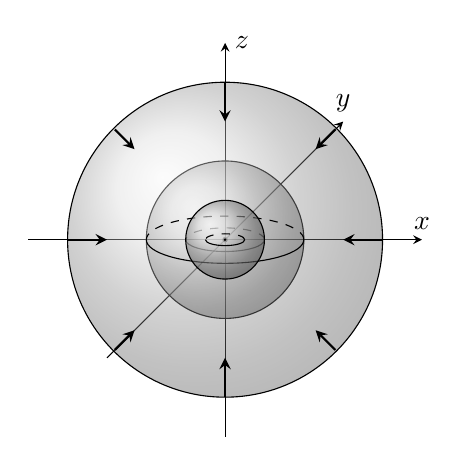
\begin{tikzpicture}[x=0.5cm,y=0.5cm,z=0.3cm,>=stealth]
            \draw[->] (xyz cs:x=-5) -- (xyz cs:x=5) node[above] {$x$};
            \draw[->] (xyz cs:y=-5) -- (xyz cs:y=5) node[right] {$z$};
            \draw[->] (xyz cs:z=-5) -- (xyz cs:z=5) node[above] {$y$};
            \shade[ball color = gray!40, opacity = 0.5] (0,0) circle (1cm);
            \draw (0,0) circle (1cm);
            \draw (-1,0) arc (180:360:1 and 0.3);
            \draw[dashed] (1,0) arc (0:180:1 and 0.3);
            \fill[fill=black] (0,0) circle (1pt);
            \shade[ball color = gray!40, opacity = 0.4] (0,0) circle (2cm);
            \draw (0,0) circle (2cm);
            \draw (-2,0) arc (180:360:2 and 0.6);
            \draw[dashed] (2,0) arc (0:180:2 and 0.6);
            %\draw[dashed] (4,0) arc (60:120:8);
            %\draw (-4,0) arc (240:300:8);
              
            \shade[ball color = gray!40, opacity = 0.6] (0,0) circle (0.5cm);
            \draw (0,0) circle (0.5cm);
            \draw (-0.5,0) arc (180:360:0.5 and 0.15);
            \draw[dashed] (0.5,0) arc (0:180:0.5 and 0.15);
            \fill[fill=black] (0,0) circle (0.5pt);
            \draw [black, -stealth, thick] (0,4) -- (0,3);
            \draw [black, -stealth,thick] (2.8,2.8) -- (2.3,2.3);
            \draw [black, -stealth,thick] (4,0) -- (3,0);
            \draw [black, -stealth,thick] (0,-4) -- (0,-3);
            \draw [black, -stealth,thick] (-4,0) -- (-3,0);
            \draw [black, -stealth,thick] (-2.8,2.8) -- (-2.3,2.3);
            \draw [black, -stealth,thick] (2.8,-2.8) -- (2.3,-2.3);
            \draw [black, -stealth,thick] (-2.8,-2.8) -- (-2.3,-2.3);
        \end{tikzpicture}
        \caption{Shrinking spheres of dimension 2}
    \end{figure}
    \item \textbf{Evolution of Graphs}: Let $ f : \R^{n} \to \R $ be a smooth function. The graph of $ f $ in $ \Rn $, 
    \[ \mathcal{M} = \{(x,f(x)) \in \Rn :  x \in \R^{n} \} \]
    is a smooth hypersurface. The mean curvature vector at $ (x,f(x)) $ for the hypersurface can be calculated to be,
    \[ \sqrt{1+ |\nabla f|^{2}} \, \text{div} \left( \frac{\nabla f}{\sqrt{1+ |\nabla f|^{2}}} \right).\]
    Ecker and Huisken proved in \cite{ecker1989mean} that graphs evolving under the mean curvature flow remain graphs. So a family of graphs $ \mathcal{M}_{t} = \{(x,f_{t}(x)) :  x \in \Rn\} $ with the condition 
    \[ \frac{\partial}{ \partial t}f_{t}(x) = \sqrt{1+ |\nabla f_{t}|^{2}} \, \text{div} \left( \frac{\nabla f_{t}}{\sqrt{1+ |\nabla f_{t}|^{2}}} \right) \]
    is a solution of the mean curvature flow. 
    \item \textbf{Minimal surfaces}: Minimal surfaces are the critical points of the volume functional. A hypersurface $ \mathcal{M} $ is said to be a \textbf{minimal hypersurface} if it satisfies $ H(x) = 0 $ for all $ x \in \mathcal{M}  $. Hence, minimal hypersurfaces are stationary solutions of the mean curvature flow. 
    \item \textbf{Products of solutions with Euclidean space}
    : Suppose $ \mathcal{M}_{t}^{n} \subset \Rn $ is a solution of the mean curvature flow. It is easy to verify that mean curvature vector of the product $ \mathcal{M}_{t}^{n} \times \R^{m} \subset \R^{n+1} \times\R^{m}  $ is given by 
    \[ \vec{H}(x,y) = (H(x) \nu(x), 0), \]
    which implies that the time-parametrized product $ \mathcal{N}_{t} = \mathcal{M}_{t} \times \Rn $ is a solution of the mean curvature flow as well.
    \begin{figure}[h]
        \centering
        \begin{tikzpicture}[x=0.5cm,y=0.5cm,z=0.3cm,>=stealth]
            \coordinate (O) at (0,0,0);
              \coordinate (A) at (2,0,0);
              \coordinate (B) at (0,2,0);
              \coordinate (C) at (0,0,2);
              \draw[->] (xyz cs:x=-5) -- (xyz cs:x=5) node[above] {$x$};
              \draw[->] (xyz cs:y=-5) -- (xyz cs:y=5) node[right] {$z$};
              \draw[->] (xyz cs:z=-5) -- (xyz cs:z=5) node[above] {$y$};
            %\draw[-latex] (O) -- (A) node[below] {$y$};
            %\draw[-latex] (O) -- (B) node[above] {$z$};
            %\draw[-latex] (O) -- (C) node[below] {$x$};
            \node[cylinder, draw, shape aspect=0.3, 
              cylinder uses custom fill, cylinder end fill=gray!50, 
              minimum height=0.7cm,
              cylinder body fill=gray!25, opacity=0.5, 
            scale=5, rotate=90]{};
            \draw [black, -stealth] (1.25,3.55) -- (0.5,3.55);
            \draw [black, -stealth] (-1.25,3.55) -- (-0.5,3.55);
            %\draw [-stealth] 
        \end{tikzpicture}
        \caption{Cylinder $ S^{1} \times \R $}
    \end{figure}  
\end{enumerate}
\subsection{Mean curvature flow as gradient of the area functional}

Let $ \mathcal{M}_{0} \subset \Rn $ be a smooth hypersurface and $ X: M^{n} \times (-\epsilon, \epsilon) \to \Rn $ be a variation with $ X(\cdot,0) = \mathcal{M}_{0} $. Considering area as a function of time over the variation, we get \begin{equation}
    \frac{d}{dt}\text{Area}( \mathcal{M}_{t}) = \int_{ \mathcal{M}_{t}} \left< \partial_{t}X, H \nu \right> 
\end{equation}
Using this, the gradient of the area functional is 
	\[ \nabla \text{Area} = H \nu \]
	so the most efficient way to reduce the volume is to choose the variation so that 
	\[ \partial_{t}X = -\nabla \text{Area} = -H \nu \]
	which is the mean curvature flow. In particular, we get the following equation for evolution of area under mean curvature flow,
	\[ \frac{d}{dt} \text{Area}( \mathcal{M}_{t}) =  - \int_{\mathcal{M}_{t}}H^{2}\]
which is the steepest descent of area in the space of hypersurface up to speed-parametrization. 
\subsection{Short-time existence}
The following theorem about the uniqueness and existence of mean curvature flow is proved in \cite{andrews2022extrinsic}. 
\begin{thm}
    Short time existence : Let $ X_{0}: M^{n} \to \Rn $ be a smooth immersion of a compact manifold without boundary. There exists an $ \epsilon >0 $ and a smooth solution $ X : M^{n} \times [0, \epsilon) \to \Rn$ to MCF, with $ X( \cdot, 0) = X_{0} $. Moreover, the solution is unique.
\end{thm}

\section{Maximum principle}\label{max}
We can extend the maximum principle on Euclidean space to general Riemannian manifolds in the following fashion. 
\begin{lemma}[Scalar maximum principle]
    Let $ g(t) \in [0,T) $ be a $ 1 $-parameter family of Riemannian metrics on a closed manifold $ \mathcal{M}^{n} $ and $ \beta : \mathcal{M}^{n} \times [0,T) \to \R $ be a locally bounded function. Let $ u : \mathcal{M}^{n} \times [0,T) \to \R$ be a $ C^{2} $ function satisfying the following inequality 
    \[ \frac{ \partial}{ \partial t}u(x,t) \ge \Delta_{g(t)}u + \beta u\]
    If $ u(x,0) \ge 0 $ for all $ x \in \mathcal{M}^{n}$, then $ u(x,t) \ge 0 $ for all $ (x,t) \in \mathcal{M}^{n} \times [0,T) $.
\end{lemma}

\begin{proof}
    
\end{proof}

The above maximum principle can be further extended to tensors. This was done by Hamilton in \cite{hamilton1982three} in the context of Ricci flow. Let $ M = M_{ij}dx^{i}\otimes dx^{j} $ be a symmetric $ 2 $-tensor. We say $ M $ is non-negative if $ v^{T}Mv = M_{ij}v^{i}v^{j} \ge 0 $ for all vectors $ v $. Let $ N_{ij} = p(M_{ij},g_{ij}) $ be a tensor formed by contracting products of $ M_{ij} $ with itself using the metric. Also suppose that whenever $ v $ is a null-eigenvector of $ M_{ij} $ (i.e. $ M_{ij}v^{j} = 0 $), we have $ N_{ij}v^{i}v^{j} \ge 0 $. Then the following maximum principle holds

\begin{lemma}[Tensor maximum principle]
	Let $ g(t) \in [0,T)  $ be a $ 1 $-parameter family of Riemannian metrics on a closed manifold $ \mathcal{M}^{n} $. Let $ M_{ij} $ be a symmetric non-negative tensor evolving by the equation 
	
        \[ \frac{ \partial}{ \partial t}M_{ij} = \Delta M_{ij} + N_{ij}  \text{ for all } (x,t) \in  \mathcal{M}^{n} \times [0,T) \]
	where $ N_{ij} = p(M_{ij},g_{ij}) $ satisfies the null-eigenvector condition above. If $ M $ is non-negative at $ t=0 $, then it remains non-negative on $ [0,T) $.
\end{lemma}

\subsection{Applications to mean curvature flow}

The tensor maximum principle can be used to prove that convexity is preserved under mean curvature flow. 

\begin{lemma}
    If 
\end{lemma}
\section{Evolution equations}
To understand the properties of mean curvature flow it is essential to know the evolution of geometric quantities of the hypersurface. Let $X : M^n \times I \to \R^{n+1}$ be a smooth solution of mean curvature flow, so 
\[ \dou_t X(x,t) = \overrightarrow{H}(x,t)  = -H(x,t)\nu(x,t)\]
Let $\{x^i\}$ be a local coordinate in $M^n$. Then the induced metric on the hypersurface is given by $g = X^*(\delta)$ where $\delta$ is the flat metric on $\R^{n+1}$. This gives
\[ g_{ij} = \delta(X_*(\dou_i),X_*(\dou_j)) = \left\langle  \frac{\dou X}{\dou x^i}, \frac{\dou X}{\dou x^j} \right\rangle  \]
\begin{lemma} Let $X: M^n \times I \to \R^{n+1}$ be a solution of mean curvature flow. Then the evolution equation of metric, normal, second fundamental form, and mean curvature is given by
\begin{equation}
    \dou_t g_{ij} = -2Hh_{ij}
\end{equation}
\begin{equation}
\dou_t \nu  = \nabla H
\end{equation}
\begin{equation}
\dou_t h_{ij} = \Delta h_{ij} - 2Hh_{il}g^{lm}h_{mj}+|A|^2h_{ij}
\end{equation}
\begin{equation}
    \dou_t H = \Delta H + |A|^2H \label{dtH}
\end{equation}
\end{lemma}
\begin{proof}
1. In local coordinates we have 
\begin{align*}
    \dou_tg_{ij} & = \partial_{t} \left\langle \partial_{i}X, \partial_{j}X \right\rangle \\
& = \left\langle \partial_{i}(\partial_{t}X), \partial_{j}X \right\rangle + \left\langle \partial_{i}X, \partial_{t}(\partial_{j}X) \right\rangle\\
& = \left\langle \partial_{t}(-H \nu), \partial_{j}X \right\rangle + \left\langle \partial_{i}X, \partial_{j}(-H \nu)\right\rangle \\
& = -H \left\langle \partial_{t} \nu, \partial_{j}X\right\rangle  - H \left\langle \partial_{i}X, \partial_{t}\nu\right\rangle \\
& = -2Hh_{ij}
\end{align*}
2. Since $\langle \nu, \nu \rangle = 1$, we have $2\langle \partial_{t}\nu, \nu \rangle = 0$, so the vector $\partial_{t}\nu$ is in the tangent plane of the hypersurface. We can write it as a linear combination of tangent vectors $\{\partial_{j}X\}$ to get
\begin{align*}
\partial_{t}\nu &= \left\langle \partial_{t}\nu, \partial_{i}X \right\rangle \partial_{j}Xg^{ij} = - \left\langle \nu, \partial_{i}X\left( \partial_{t}X \right) \right\rangle\partial_{j}X g^{ij} \\
& = \left\langle \nu, \partial_{i}\left( H \nu \right) \right\rangle \partial_{j}Xg^{ij}\\
& = \partial_{i}H \partial_{j}X g^{ij} + H \left\langle \nu, \partial_{i}\nu\right\rangle \partial_{j}Xg^{ij}\\
& = \partial_{i}H\partial_{j}Xg^{ij} = \nabla H
\end{align*}
3. From the relations \[
\partial_{i}\partial_{j}X = \Gamma^{k}_{ij}\partial_{k}X	-h_{ij}\nu \quad \text{ and } \quad\partial_{j}\nu = h_{jl}g^{lm}\partial_{m}X\] we get 
\begin{align*}
\partial_{t} h_{ij} & = - \partial_{t} \left\langle\partial_{i}\partial_{j}X ,\nu\right\rangle\\
& = \left\langle\partial_{i}\partial_{j}(H \nu), \nu \right\rangle - \left\langle \partial_{i}\partial_{j}X, \partial_{l}H \partial_{m}Xg^{lm}\right\rangle \\
& = \partial_{i}\partial_{j}H + H \left\langle \partial_{i}\left( h_{jm}g^{ml} \partial_{l}X \right), \nu \right\rangle -\left< \Gamma_{ij}^{k}\partial_{k}X-h_{ij}\nu,\partial_{l}H \partial_{m}Xg^{lm} \right>\\
& = \partial_{i}\partial_{j}H - \Gamma_{ij}^{k}\partial_{k}H + Hh_{jm}g^{ml}\left< \Gamma_{il}^{p}\partial_{p}X- h_{il}\nu, \nu \right> \\
& = \nabla_{i}\nabla_{j}H- Hh_{il}g^{lm}h_{mj}.
\end{align*}
4. Utilizing the previous evolution equation with product formula of derivatives, 
\begin{align*}
\dou_t H &= \dou_t(g^{ij}h_{ij}) = (\partial_{t}g^{ij})h_{ij}+ g^{ij}\partial_{t}h_{ij}\\
& = -g^{ik}(\partial_{t}g_{kl})g^{lj}h_{ij}+ g^{ij}(\Delta h_{ij} - 2Hh_{il}g^{lm}h_{mj}+|A|^2h_{ij})\\
& = -g^{ik}(-2Hh_{kl})g^{lj}h_{ij}+ \Delta(g^{ij}h_{ij}) - 2Hg^{ij}g^{lm}h_{il}h_{mj}+|A|^2H\\
& = 2H|A|^2 + \Delta H - 2H|A|^2 + |A|^2H\\
& =  \Delta H+ |A|^2H.
\end{align*}
\end{proof}
\begin{corollary}
If mean curvature is positive everywhere on the initial hypersurface, then it remains so throughout the flow.
\end{corollary}
\begin{proof}
We apply maximum principle to the evolution equation of $H$.
\end{proof}
\begin{remark}
This property of mean curvature holds even when the hypersurface is embedded in an arbitrary Riemannian manifold with positive Ricci curvature. 
\end{remark}
\section{The Avoidance Principle}

Let $X_i : M^n_i \times  [0,T) \to \R^{n+1}, i = 1,2 $ be properly immersed solutions to mean curvature flow such that at least one of  $ M^n_1$ or $M^n_2$ is compact. 
If the hypersurfaces are disjoint initially, i.e. $X_1(M^{n_1},0)\cap X_2(M^n_2,0) = \phi$, then they remain so. Define the distance function $d: M^n_1 \times M^n_2 \times  [0,T) \to \R$ between the solutions by \[
d(x,y,t) = |X_2(y,t) - X_1(y,t)|
.\] 
as a function of time. From the assumption of compactness $d_0 \define \inf_{(x,y) \in M^n_1 \times M^n_2} d(x,y,0) >0$
\begin{figure}[h]
\centering
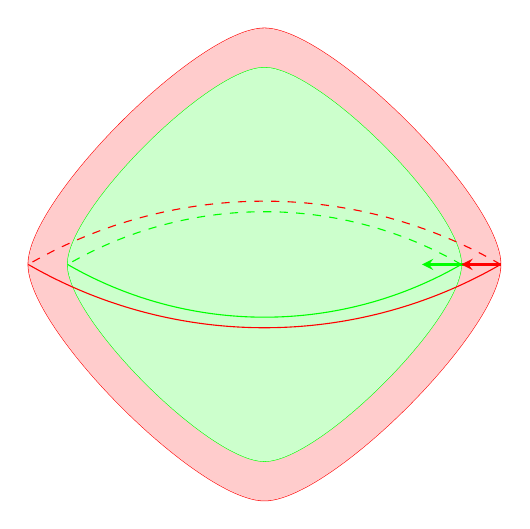
\begin{tikzpicture}
    \draw [red] plot [smooth cycle] coordinates {(3,0)(0,3)(-3,0)(0,-3)};
    %\draw [red](0,0) circle (3cm);
    \fill [red!20] plot [smooth cycle] coordinates {(3,0)(0,3)(-3,0)(0,-3)};
    
    
    \draw [green] plot [smooth cycle] coordinates {(2.5,0)(0,2.5)(-2.5,0)(0,-2.5)};
    \fill [green!20] plot [smooth cycle] coordinates {(2.5,0)(0,2.5)(-2.5,0)(0,-2.5)};
    \draw [dashed,green] (2.5,0) arc (60:120:5cm);
    \draw [green] (-2.5,0) arc (240:300:5cm);
    \draw [thick,green][-stealth](2.75,0) -- (2,0);
    \draw [thick,red][-stealth](3,0) -- (2.5,0);
    \draw [dashed,red] (3,0) arc (60:120:6cm);
    \draw [red] (-3,0) arc (240:300:6cm); 
\end{tikzpicture}
\caption{Disjoint hypersurfaces flowing under MCF}
\end{figure}
\begin{thm}
If $X_1$ and $X_2$ are solutions to mean curvature flow on closed manifolds with $ d_{0}>0$, then $ d(x,y,t)>0$ for all $ x,y,t$. In particular, if $ X_1(x,0) \neq X_2(y,0)$ for all $x \in M^n_1  $ and $ y \in M^n_2$, then $ X_1(x,t) \neq X_2(y,t)$ for all $ x \in M^{n}_1$, $y \in  M^n_2$ and $ t \in  [0,T)$. 
\end{thm}
\begin{proof}
Assume on the contrary $ d(x,y,t)$ is not everywhere strictly greater that $ d_{0} $. Then there exists a $ t_{0} $ such that $ d(x_{0},y_{0},t_{0}) = d_{0} - \delta $
\end{proof}
\begin{remark}
From the proof we can conclude that the distance between the hypersurfaces is a non-decreasing function. Another way to see this is that $ d_{t} $ satisfies a heat-type parabolic equation 
    \[ TO\, DO \]
 on which maximum principle is applicable. 
\end{remark}
\begin{proof} Fix $\epsilon > 0$ and suppose that $e ^{\epsilon (1+t)}d(x,y,t)$ is not strictly greater than $d_0$. That is there exists a time $ t_0 > 0$ such that $e^{\epsilon(1+ t)}d(\cdot, \cdot, t)$ reaches $ d_0$. That is,\[
e^{\epsilon(1+t)}d(\cdot,\cdot,t)> 0 \quad \text{ for } t < t_0
.\]  and \[
e^{\epsilon(1+t)}d(x_0,y_0,t_0) = d_0 \quad \text{ for some }(x_0,y_0) \in   M^n_1 \times  M^n_2		
.\] Then \[
\pt (e^{\epsilon(1+t)}d)|_{(x_0,y_0,z_0)} \le 0 
.\] Let $D$ denote the Euclidean directional derivative, by $ \nabla_i$ the covariant derivative induced on $M^n_i$ by $X_i$, and by $\nabla $ the covariant derivative on $ M^n_1 \times  M^n_2$ induced by $ \nabla_1$ and $ \nabla_2$, we find \[
\nabla^2
.\] 

\end{proof}
\begin{remark}
We can phrase the avoidance principle as : disjointness is an immortal property and jointness is an ancient property.
\end{remark}


\section{Long time existence}

In this subsection we will prove that blowing up of second fundamental form is the only obstruction for continuing the flow. The proof goes by contrapositive, relying on the Bernstein type estimates. This technique is very similar to the one Hamilton used for Ricci flow \cite{hamilton1982three}. A solution of the mean curvature flow $ X : M^{n} \times [0,T) \to \Rn $ is said to be \textbf{maximal}  if given any other solution $ Y : M^{n} \times [0,S) \to \Rn $ which coincides with $ X $ for $ t \in [0,T) \cap [0,S) $ we have $ T \ge S $. Such a $ T $ is said to be the \textbf{maximal time} for $ X $. 

\begin{thm}\label{longtimeexistence}
    Let $ X : M^{n} \times [0,T) \to \Rn $ be a solution of the mean curvature flow with $ M^{n} $ compact. If $ X $ is maximal then $ T< \infty $ and 
    \[ \sup_{M^{n} \times [0,T)} |A| = \infty.\]
\end{thm}

Before jumping into the proof we need a general notation for complicated tensor expressions occurring in evolution equations. 
\begin{defn}
    Given any two tensors $ A $ and $ B $, we write $ A * B $ to denote any linear combination of tensors formed by contraction on $ A_{i_{1} \dots i_{k}}^{a_{1} \dots a_{p}}B_{j_{1} \dots j_{l}}^{b_{1} \dots b_{q}} $ with $ g $ or $ g^{-1} $. The iterated product $ A * B * C $ can be viewed as $ A * (B * C) $ which is associative so can be written without brackets. Also, denote the multifold product $ \underbrace{A * \dots * A}_{p-\text{times}}$ by $ A^{*p} $. The Gauss equation in this notation yields $ \text{Rm} = A * A $ which after differentiation gives $ \nabla \text{Rm} = A * \nabla A $. 
\end{defn}

The following lemma will be necessary to find out time derivative of covariant derivatives and gives the commutator relation between it. 
\begin{lemma}
    Let $ S $ be a tensor with evolution equation given by 
    \[ \partial_{t} S = \Delta S + T \]
    where $ T $ is another tensor of same rank. Then the evolution equation of the covariant derivative is \begin{equation}
        \partial_{t}\nabla S = \Delta \nabla S + A * A  * \nabla S + A * \nabla A * S + \nabla T.
    \end{equation}
\end{lemma}
\begin{proof}
    Recall the time evolution of Christoffel symbol is given by     
    \begin{equation}
        \partial_{t}\Gamma_{ij}^{k} = \frac{1}{2}g^{kl}(\nabla_{i}\partial_{t}g_{jl}+ \nabla_{j}\partial_{t}g_{il}-\nabla_{l}\partial_{t}g_{ij}).
    \end{equation}
    Substituting $ \partial_{t}g_{ij} = -2Hh_{ij} $ we get 
    \[ \partial_{t}\Gamma_{ij}^{k} = -g^{kl}(\nabla_{i}(Hg_{jl})+ \nabla_{j}(Hg_{il})-\nabla_{l}(h_{ij})) = A * \nabla A. \]
    Consider the commutator \begin{align*}
        \partial_{t}\nabla S & = \nabla \partial_{t}S + \partial_{t}\Gamma *S \\
        & = \nabla(\Delta S+T) + A * \nabla A * S \\
        & = \Delta \nabla S + \nabla \Rm * S + \Rm * \nabla S  + \nabla T + A * \nabla A * S \\
        & = \Delta \nabla S + A * A  * \nabla S + A * \nabla A * S + \nabla T
    \end{align*}
    where we have used the Ricci identity $ [\nabla, \Delta]S = \nabla \Rm * S + \Rm * \nabla A $.
\end{proof}



\begin{lemma}
    The evolution equation of higher gradient of second fundamental form is given by 
    \begin{equation}
        \partial_{t}\nabla^{m}A = \Delta \nabla^{m}A + \sum_{i+j+k =m}^{}\nabla^{i}A* \nabla^{j}A*\nabla^{k}A 
    \end{equation}
    where $ m \in \N \cup \{0\} $. Further, the norm of the gradient satisfies 
    \begin{equation}
        \partial_{t}|\nabla^{m}A|^{2} = \Delta |\nabla^{m}A|^{2}- 2 |\nabla^{m+1}A|^{2} +\sum_{i+j+k =m}^{}\nabla^{i}A* \nabla^{j}A*\nabla^{k}A* \nabla^{m}A \label{normnablaA}
    \end{equation}
    where $ m \in \N \cup \{0\} $.
    
\end{lemma}
\begin{proof}
    We induct on $ m $. For base case $ m = 0 $, the second fundamental form evolution equation is 
    \begin{align*}
        \partial_{t} A & = \Delta A -2H A^{2} + |A|^{2}A \\
        & = \Delta A + A*A*A. 
    \end{align*}
    Now suppose the equation holds for $ m $, then for $m +1 $ we have \begin{align*}
        \partial_{t}\nabla^{m+1}A & = \nabla \partial_{t} (\nabla^{k}A) + (\partial_{t}\Gamma)* \nabla^{m}A \\
        & = \nabla \left(\Delta \nabla^{m}A + \sum_{i+j+k=m}^{}\nabla^{i}A * \nabla^{j}A * \nabla^{k}A\right) + A * \nabla A * \nabla^{m}A \\
        & = \Delta \nabla^{m+1}A + \nabla \Rm * \nabla^{m}A + \Rm* \nabla^{m+1}A + \sum_{i+j+k =m+1}^{}\nabla^{i}A* \nabla^{j}A*\nabla^{k}A \\
        & = \Delta \nabla^{m+1}A + \sum_{i+j+k =m+1}^{}\nabla^{i}A* \nabla^{j}A*\nabla^{k}A
    \end{align*}
    using Ricci identity and Gauss equation $ \Rm = A*A $. For the norm, we get \begin{align*}
        \partial_{t}|\nabla^{m}A|^{2} = 2\left<\partial_{t}\nabla^{m}A, \nabla^{m}A  \right> + A*A* \nabla^{m}A * \nabla^{m}A
    \end{align*}
    where the second term comes from time derivative $ \partial_{t}g^{ij} = -2Hh^{ij} = A*A $. This simplifies to \begin{align*}
        \partial_{t}|\nabla^{m}A|^{2} & = 2\left< \Delta \nabla^{m}A + \sum_{i+j+k=m}^{}\nabla^{i}A * \nabla^{j}A* \nabla^{k}A, \nabla^{m}A  \right> + A*A*\nabla^{m}A * \nabla^{m}A \\
        & = 2\left< \Delta \nabla^{m}A , \nabla^{m}A \right> + \sum_{i+j+k=m}^{}\nabla^{i}A * \nabla^{j}A* \nabla^{k}A \nabla^{m}A \\
        & = \Delta|\nabla^{m}A|^{2} - 2|\nabla^{m+1}A|^{2} + \sum_{i+j+k=m}^{}\nabla^{i}A * \nabla^{j}A* \nabla^{k}A* \nabla^{m}A
    \end{align*}
\end{proof}
We can consider maximum principle on the previous lemma. This gives control of derivates of the second fundamental form based on the bound of second fundamental form. 

\begin{lemma}
    Let $ X : M^{n} \times [0,T) \to \Rn $ be a solution of the mean curvature flow with $ M^{n} $ compact. Suppose that $ T < \infty $ and $ C_{0} = \sup_{M^{n} \times [0,T)}|A| < \infty $. Then for each $ m \in \N $ there exists a constant $ C_{m} < \infty $ depending only on initial manifold such that \begin{equation}
        \sup_{M^{n} \times [0,T)} |\nabla^{m}A| \le C_{m}.
    \end{equation}
\end{lemma}

\begin{proof}
    From \cref{normnablaA}, we can estimate \begin{align*}
        \partial_{t}|\nabla^{m}A|^{2} \le \Delta|\nabla^{m}A|^{2} - 2|\nabla^{m+1}A|^{2} + C_{n,m}\sum_{i+j+k=m}^{}|\nabla^{i}A|  |\nabla^{j}A|| \nabla^{k}A|| \nabla^{m}A|
    \end{align*}
    where $ C_{n,m}< \infty $ only depends on $ n $ and $ m $. We now proceed by induction on $ m $. Suppose that for $ l \in \{1, \dots, m-1\} $ we have 
    \[ \sup_{\mathcal{M} \times [0,T)} |\nabla^{l}A|^{2} \le C_{l}\]
    for some constants $ C_{l} < \infty$. From the previous relation, \begin{align}
        \partial_{t}|\nabla^{m}A|^{2} & \le \Delta |\nabla^{m}A|^{2} - 2 |\nabla^{m+1}A|^{2} + C_{n,m} \left( |A|^{2} |\nabla^{m}A|^{2} + \sum_{\substack{i+j+k=m \\
        i,j,k \le m-1}}^{}|\nabla^{i}A||\nabla^{j}A||\nabla^{k}A||\nabla^{m}A|  \right) \nonumber \\
        & \le \Delta|\nabla^{m}A|^{2}+ C_{n,m}C_{0}^{2}|\nabla^{m}A|^{2} + c_{m}|\nabla^{m}A|  \nonumber \\
        & \le \Delta|\nabla^{m}A|^{2} + 2C_{n,m}C_{0}^{2}|\nabla^{m}A|^{2} + \frac{c_{m}}{4C_{0}^{2}C_{n,m}} \label{nablam}
    \end{align}
    using the induction hypothesis. To absorb the $ |\nabla^{m}A|^{2} $ term on the right-hand side consider the inequality for $ m-1 $, \begin{align}
        \partial_{t}|\nabla^{m-1}A|^{2} &\le \Delta |\nabla^{m-1}A|^{2} - 2|\nabla^{m}A|^{2} + C_{n,m-1} \sum_{i+j+k=m-1} |\nabla^{i}A||\nabla^{j}A| |\nabla^{k}A| |\nabla^{m-1}A| \nonumber\\
        & \le \Delta|\nabla^{m-1}A|^{2} - 2|\nabla^{m}A|^{2} + c_{m-1} \label{nablam1}.
    \end{align}
    Multiplying \cref{nablam1} by $ C_{n,m}C_{0}^{2} $ and adding to \cref{nablam}, \begin{align*}
        \partial_{t}\left( |\nabla^{m}A|^{2}+ C_{n,m}C_{0}^{2}|\nabla^{m-1}A|^{2} \right) & \le \Delta\left( |\nabla^{m}A|^{2}+ C_{n,m}C_{0}^{2}|\nabla^{m-1}A|^{2} \right) + \frac{c_{m}}{4C_{0}^{2}C_{n,m}} + c_{m-1}C_{n,m}C_{0}^{2}.
    \end{align*}
    Now by maximum principle 
    \[ \sup_{\mathcal{M}^{n} \times [0,T)}\left( |\nabla^{m}A|^{2}+ C_{n,m}C_{0}^{2}|\nabla^{m-1}A|^{2} \right) \le \left( \frac{c_{m}}{4C_{0}^{2}C_{n,m}} + c_{m-1}C_{n,m}C_{0}^{2} \right)T \]
    which implies 
    \[ \sup_{\mathcal{M} \times [0,T)} |\nabla^{m}A|^{2} \le C_{m}\]
    for some constant $ C_{m} < \infty $.
    
\end{proof}
We can improve the higher order covariant derivative bound to include a time factor as well. In fact the following lemma will imply rapid decrease in the norm of higher covariant derivatives of second fundamental form with respect to time. 

\begin{lemma}
    Let $ X : M^{n} \times [0,r^{2}] \to \Rn  $ be a solution of the mean curvature flow. Suppose there exists a constant $ C_{0} < \infty$ such that 
    \[ \sup_{\mathcal{M}^{n} \times [0,r^{2}]} |A|^{2} \le C_{0}r^{-2}. \]
    Then for each $ m \in \N $, there exists a constant $ C_{m} $ depending only on $ n, \mathcal{M}_{0},C_{0} $ such that 
    \[ \sup_{\mathcal{M} \times [0,r^{2}]} |\nabla^{m}A|^{2} \le C_{m}r^{-2}t^{-m} .\]

    
\end{lemma}
\begin{proof}
    The proof goes through induction on $ m $. The base case $ m=0 $ is our hypothesis, 
\end{proof}

\begin{remark}
    The parabolic nature of the mean curvature flow shows up here as the dimension of time is 
\end{remark}
\begin{proof}[ of \cref{longtimeexistence}]
    Assume on the contrary that $ \sup_{M^{n} \times [0,T)}|A|^{2} \le C $. Our aim is to prove that the manifold $X(\cdot, t)= \mathcal{M}_{t} $ converges to a smooth limit $ \mathcal{M}_{T} $ as $ t \to T $ which will give a contradiction by applying short time existence of mean curvature flow at $ t  = T $. 
\end{proof}










\section{Huisken's theorem}

Huisken's theorem proves the convergence of compact, uniformly convex hypersurface to sphere under Mean curvature flow in finite time. 
\begin{thm}
Let $ X : M^{n} \times [0,T) \to \Rn  $, $ n \ge 2 $ be a maximal solution of MCF such that $ M^{n} $ is compact and $X_{0} = X(\cdot, 0)$ is convex embedding. Then $ X_{t} = X(\cdot,t) $ is a convex embedding for all $ t>0 $ and $ X_{t} $ converges to a point $ p \in \Rn $ as $ t \to T $. Further the rescaled embeddings $ \tilde{X}_{t} : M^{n} \to \Rn $ defined by 
            \[ \tilde{X}_{t}(x) \define \frac{X_{t}(x)-p}{\sqrt{2n(T-t)}}\]
converge uniformly in the smooth topology to a smooth embedding whose image coincides with the unit sphere $ S^{n} $.
\end{thm}
\subsection{Pinching estimate}

The quantity $ \frac{|A|^{2} - \frac{H^{2}}{n}}{H^{2}} = \frac{1}{n} \sum_{i<j}^{} \left( \frac{\kappa_{i}}{H}- \frac{\kappa_{j}}{H} \right)^{2}  $ is scaling invariant and measures the roundness of the hypersurface. If we compute the evolution equation we get \begin{equation}
EQUATION
\end{equation} 
but the maximum principle is not directly applicable because of the positive last term. So we do not directly get a pointwise $ L^{\infty} $ bound we do the next best thing possible which is $ L^{p} $ bounds. After obtaining this there is a sophisticated iteration argument developed by Stampacchia which allows us to produce an $ L^{\infty} $ estimate. See  \href{https://youtu.be/a577KPiOoxw?t=1790}{here}
\begin{thm}
There exists constants $ \delta $ and $ C_{0} < \infty $ depending only on $ \mathcal{M}_{0} $ such that 
\[ |A|^{2} - \frac{H^{2}}{n} \le C_{0}H^{2-\delta} \]
for $ t \in (0,T] $.

\end{thm}
Let $ f_{\sigma} = \frac{|A|^{2}- \frac{H^{2}}{n}}{H^{2-\sigma}} = \left(\frac{|A|^{2} - \frac{H^{2}}{n}}{H^{2}}\right)H^{\sigma}$, then the evolution equation of $ f_{\sigma} $ is 
\begin{lemma}
The evolution of $ f_{\sigma} $ is given by \begin{align*}
    \frac{ \partial}{ \partial t}f_{\sigma} & = 
\end{align*}
\end{lemma}
\begin{comment}
    (Huisken' remark on this from the lecture series : the bad term can only be controlled using integral estimates \href{https://www.mfo.de/about-the-institute/staff/prof-dr-gerhard-huisken/lectures/mean-curvature-flow/lecture-3}{58 min mark} )

(Sinestrari intuition about Stampacchia iteration : \href{https://youtu.be/XvUGowx9WNo?t=2119}{yt link})
\end{comment}
\begin{comment}
    
\subsection{Width-pinching}

Let $ \Omega  \subset \Rn  $ be a compact, convex body with  boundary $  \mathcal{M}  = \partial \Omega$. %such that $ \mathcal{M} $ is locally uniformly convex. 
%This allows us to define inverse of the Gauss map on the hypersurface $ \mathcal{M} $. 
Define the support function $ \sigma : S^{n} \to \R $ as follows 
\[ \sigma(z) \define \sup_{x \in \Omega}\left< x,z \right> .\]
Using this we define the width function of $ \Omega $ by 
\[ w(z) = \sigma(z)+ \sigma(-z) \qquad \text{ for all } z \in S^{n} \]
which as the name suggests measures the width of $ \Omega  $ in the direction $ z$. Let $ w_{+} $ and $ w_{-} $ denote the maximum and minimum width. It is easy to see that maximum width is the diameter of $ \Omega $, so 
\[ w_{+} = \sup_{x,y \in \Omega}||x-y||. \]
If $ \mathcal{M}$ is smooth uniformly convex hypersurface, then we can write the support function in terms of Gauss map $ G : \partial \Omega \to S^{n} $ as 
\[ \sigma(z) = \left< G^{-1}(z), z \right>, \] so 
\[ \sigma(G(z)) = \left< z,G(z) \right>.\]

It is a lemma by Andrews that the pinching of principal curvatures implies the pinching of the widths, which will be later important to prove convergence of the hypersurface into a point. 
\begin{lemma}
Let $ \Omega \subset \Rn $, $ n \ge 2 $ be a uniformly convex body with compact, smooth boundary $ \mathcal{M} = \partial \Omega $. Suppose the principal curvatures of $ \mathcal{M} $ are pinched by a constant $ C < \infty $, i.e. $ \kappa_{n}(x) \le C \kappa_{1}(x) $ for all $ x \in \mathcal{M}  $. Then the widths of $ \mathcal{M} $ are pinched by the same constant, so 
\[ w_{+} \le C w_{-} \]
\end{lemma}
\begin{proof}
We will first prove it for $ n=2 $, which presents the main idea. Let $ e  \in S^{2}$ be unit vector in $ \R^{3} $ and (TO DO LATER) 
\end{proof}

We know the solution of MCF of spheres, so it will be useful to relate the widths of the hypersurface to the spheres inscribed and circumscribed about it. Let $$ \rho_{+} \define \inf\{r : \Omega \subset B_{r}(x) \text{ for some }x \in \R^{n}\}$$ denote the circumradius and 
\[ \rho_{-} \define \sup\{B_{r}(X) \subset \Omega \text{ for some }x \in \R^{n}\} \]
denote the inradius radius. There is also a relation between inscribed and circumscribed radius to widths of the hypersurface as given by the following lemma
\begin{lemma}
On any bounded convex body $ \Omega \subset \Rn $, 
\[ \rho_{+} \le \sqrt{n+1}w_{+} \quad \text{ and } \quad \rho_{-} \ge \frac{1}{n+2}w_{-}.\]
\end{lemma}
\begin{remark}
These are not the best bounds however they are sufficient for our purpose.
\end{remark}

Combining the two lemmas, we get 
\begin{equation}
\rho_{+} \le \frac{n+2}{\sqrt{n+1}}C\rho_{-} \label{pinching}
\end{equation}

Let $ \{\mathcal{M}_{t}\}_{t \in [0,T)}$ be family of hypersurfaces flowing under MCF with maximal time $ T $ and the initial pinching constant given by
\[ C = \sup_{ \mathcal{M}_{0}} \frac{\kappa_{n}}{\kappa_{1}} \]

If we can show that $ \rho_{-} \to 0 $ as $ t \to T $, then inequality (\ref{pinching}) would imply $ \rho_{+} \to 0 $. This proves the convergence of hypersurfaces to a point. 
\begin{thm}
The inradius $ \rho_{t} $ of $ \Omega_{t} $ tends to zero as $ t \to T $. Thus, $ \mathcal{M}_{t} $ converges to some point $ p \in \Rn $ as $ t \to T $.
\end{thm}
\end{comment}

\section{Monotonicity Formula}
Let $ X :M^{n} \times I \to \R^{n+1} $ be one-parameter family of immersions flowing by mean curvature. Let $ \{x^{i}\} $ be local coordinates around a point $ p \in M $. Then the metric and second fundamental form are given by 
\[ g_{ij} = \left< \frac{\dou X}{\dou x^{i}}, \frac{\dou X}{\dou x^{j}} \right> , \qquad h_{ij} = \left<\eta, \frac{\partial^{2}X}{\dou x^{i}\dou x^{j}} \right>. \]

If we scale the solution by a factor of $ \lambda  $, defined by $ \tilde{X}(x,t) = \lambda X(x,t) $ we get the following metric and second fundamental form 

\[ \tilde{g_{ij}} = \left< \frac{\dou \tilde{X}}{\dou x^{i}}, \frac{\dou \tilde{X}}{\dou x^{j}} \right>  = \lambda^{2}g_{ij} ,\qquad \tilde{h_{ij}} = \left<\eta, \frac{\partial^{2}\tilde{X}}{\dou x^{i}\dou x^{j}} \right>  = \lambda h_{ij}\]
so the scaled mean curvature is given by $ \tilde{H} = \tilde{g}^{{ij}}\tilde{h}_{ij} = \frac{1}{\lambda}H $. This implies the scaled solutions satisfy the evolution equation

\[ \frac{\dou \tilde{X}}{\dou t} = \lambda \frac{\dou X}{\dou t} = -\lambda^{2}\tilde{H}\eta \]
or
\[ \frac{\dou \tilde{X}}{\dou (\lambda^{2}t)} = - \tilde{H}\eta \]
Hence if scale time by $ \lambda^{2} $, then $ \tilde{X} $ is also a solution of the mean curvature flow.

Mean curvature flow is invariant under parabolic scaling, i.e.  if $ X : M^{n} \times I \to \R^{n+1} $ is solution, then so is $ X_{\lambda}(x,t) = \lambda X(x,\lambda^{2}t) $. We construct a weighted area functional which is invariant under \textit{parabolic} scaling along any solution to mean curvature flow which will be monotonous.

Let $ \rho(x,t) $ be the backward heat kernel at $ (X_{0},t_{0}) $, i.e.,   \[\rho(x,t) = \frac{1}{(4 \pi (t_{0}-t))^{ \frac{n}{2}} }\cdot \exp\left( - \frac{|X(x,t)-X_{0}|^{2}}{4(t_{0}-t)} \right), \qquad t<t_{0} \]
\begin{thm}
If $ M_{t} $ is a solution of mean curvature flow for $ t< t_{0} $, then we have the formula

    \[ \frac{d}{dt} \int_{M_{t}}\rho(x,t)d \mu_{t}  = - \int_{M_{t}}\rho(x,t)\left( H- \frac{\left< X(x,t)-X_{0}, \eta \right>}{2 (t_{0}-t)} \right)^{2}d \mu_{t}\] 

\end{thm}
\begin{proof}
To simplify the formula assume that $ \left(X_{0},t_{0}\right) = (0,0) $. We know that $ \frac{d}{dt} \mu_{t} = -H^{2} \mu_{t} $, so differentiating $ \rho $ with respect to time we get,
\begin{align}
    \frac{d}{dt} \int_{M_{t}}\rho(x,t)d \mu_{t}  &= \int_{M_{t}}\rho(x,t)(-H^{2})d \mu_{t} + \int_{M_{t}} \frac{\dou}{\dou t}\rho(x,t)d \mu_{t}\nonumber \\
    & = -\int_{M_{t}}\rho(x,t)H^{2}d \mu_{t} +\int_{M_{t}}\left( \frac{\left< X(x,t), H(x,t)\eta \right>}{2(-t)}\rho(x,t) \right)d\mu_{t}\nonumber \\
    &  \qquad \qquad  + \int_{M_{t}} \left( \frac{n}{2(4 \pi)(-t)}(4 \pi)\rho(x,t) -\frac{|X(x,t)|^{2}}{4(-t)^{2}}\rho(x,t)\right)d \mu_{t}\nonumber \\ 
    & = \int_{M_{t}}\rho\left(   \frac{n}{2(-t)} +\frac{\left< X,H \eta\right>}{2(-t)}- \frac{|X|^{2}}{4(-t)^{2}} -H^{2}\right)d \mu_{t}\label{rho0}
    %& = -\int_{M_{t}}\rho \left| H \eta + \frac{X}{2(-t)}\right|^{2}d \mu_{t} + \int_{M_{t}}\rho \frac{ \left< X,H \eta \right>}{2(-t)} d \mu_{t} + \int_{M_{t}} \frac{n\rho}{2(-t)}d \mu_{t} \label
\end{align}

Now $ \Delta X = - H \eta $, using this relation for second term and divergence theorem we get 
\begin{align}
\int_{M_{t}}\rho \left< X,H \eta \right> d \mu_{t} & =  -\int_{M_{t}} \rho\left< X,\Delta X \right> d \mu_{t} \nonumber \\ 
& = - \sum_{k=1}^{n+1}\int_{M_{t}} \rho X_{k} \Delta X_{k} d \mu_{t}\nonumber \\
& = \sum_{k=1}^{n+1} \int_{M_{t}} \left< \nabla(\rho X_{k}), \nabla X_{k} \right>d \mu_{t}\nonumber \\ 
& = \sum_{k=1}^{n+1} \int_{M_{t}} \left( \left< \nabla\rho, \nabla X_{k} \right>X_{k} + \rho \left< \nabla X_{k}, \nabla X_{k} \right> \right)d \mu_{t} \label{rho1}
% & = \int_{M_{t}} \left< \nabla(\rho X), \nabla X \right>d \mu_{t}\\ 
% & = \int_{M_{t}} \left( \rho\left< \nabla X, \nabla X  \right> + \left< \nabla \rho, \nabla X \right> X \right)
\end{align}
Let $ (U,\{x^{i}\}) $ be some local coordinates on the hypersurface. In these coordinates we can write $ \nabla \rho = g^{ij} \partial_{i} \rho \partial_{j} $, so $  \left< \nabla \rho , \nabla X_{k}\right> = \nabla \rho (X_{k}) = g^{ij} (\partial_{i}\rho) (\partial_{j}X_{k}) $ which implies 
\begin{align}
\sum_{k=1}^{n+1} \left< \nabla \rho , \nabla X_{k}  \right> X_{k} & = \sum_{k=1}^{n+1}  g^{ij} (\partial_{i}\rho) (\partial_{j}X_{k}) X_{k}\nonumber \\ 
& = g^{ij}( \dou_i \rho) \left< X, \dou_j X \right>\nonumber \\
& = g^{ij} \rho \left( \frac{-\left< X, \partial_{i}X \right>}{2(-t)} \right) \left< X, \dou_j X \right>\nonumber \\
& = - \frac{\rho}{2(-t)}|X^T|^2 \label{rho2}
\end{align}
and 
\begin{equation}
\sum_{k=1}^{n+1} \rho  \left< \nabla X_{k}, \nabla X_{k} \right> = \sum_{k=1}^{n+1} \rho g^{ij} (\partial_{i} X_{k} )(\partial_{j}X_{k}) = \rho g^{ij} \left<  \partial_{i}X, \partial_{j}X \right> = \rho g^{ij}g_{ij} = n \rho \label{rho3}
\end{equation}
Substituting \cref{rho2} and \cref{rho3} into \cref{rho1} and multiplying by $ \frac{1}{2(-t)} $, we get 
\begin{equation*}
\int_{M_{t}}\rho  \frac{\left< X,H \eta \right>}{2(-t)} d \mu_{t}  = \int_{M_{t}} \rho \left( \frac{n}{2(-t)} - \frac{1}{4(-t)^2}|X^T|^2  \right) d \mu_{t} 
\end{equation*}
or 
\begin{equation}
\int_{M_{t}}\frac{n\rho}{2(-t)} d \mu_{t} = \int_{M_{t}} \rho \left(  \frac{\left< X,H \eta \right>}{2(-t)} + \frac{1}{4(-t)^2}|X^T|^2 \right)d \mu_{t}\label{rho4}
\end{equation}
where $ X^{T} $ denotes the tangential part of the vector $ X $. Substituting \cref{rho4} into \cref{rho0}
\begin{align*}
\frac{d}{dt} \int_{M_{t}}\rho(x,t)d \mu_{t}  &=  \int_{M_{t}}\rho\left(\frac{\left< X,H \eta\right>}{(-t)}- \frac{|X|^{2}}{4(-t)^{2}} -H^{2}+ \frac{1}{4(-t)^2}|X^T|^2\right)d \mu_{t}\\ 
& = -\int_{M_{t}} \rho \left( H - \frac{\left< X, \eta \right>}{2(-t)} \right)^{2} d \mu_{t}.
\end{align*}
\end{proof}

\subsection{Rescaled Monotonicity formula}\label{Type1singularity}

From section (?) we know that the curvature blows up at the maximal time $ T $  and satisfies the inequality

\[ \max_{p \in M}|A(p,t)| \ge \frac{1}{\sqrt{2(T-t)}} \]

\begin{defn}
Let $ T $ be the maximal time of existence of a mean curvature flow. If there exists a constant $ C >1 $ such that 

    \[ \max_{p \in M}|A(p,t)| \le \frac{C}{\sqrt{2(T-t)}} \]
we say the flow is developing at time $ T $ a \textit{type I singularity}.
\end{defn}

Conversely, if such a constant does not exist, that is 

\[ \limsup_{t \to T} \max_{p \in M}|A(p,t)|\sqrt{T-t} = \infty \]

we say that we have a \textit{type II singularity}. We will restrict ourselves to type I singularity for the rest of this section. 


\section{Surfaces of positive mean curvature}

From the maximum principle we know that if mean curvature of the initial hypersurface $M_0$ is positive then it will stay positive on $M_t$. 
For self-similar solutions, we know that the limiting hypersurface will satisfy the equation $H = \langle x, \nu \rangle$. 
We prove that sphere is the only compact hypersurface of positive mean curvature moving under self-similarity 
\begin{thm}
If $M^n$, $n\ge 2$, is compact with non-negative mean curvature $H$ and satisfies the equation $H = - \langle X, \nu \rangle$, then $M^n$ is a sphere of radius $\sqrt{n}$. 
\end{thm}
\begin{proof}
Suppose the hypersurface satisfies $H = -\langle X, \nu \rangle$. Let $e_1,\ldots, e_n$ be an orthonormal frame on $M^n$, then 
\begin{align}
    \nabla_{i}H & = - \left< D_{e_{i}}X, \nu \right> - \left< X, \nabla_{e_{i}}\nu \right> \nonumber \\
    & = -\left< e_{i}, \nu \right> - \left< X, \left< \nabla_{e_{i}}\nu,e_{l} \right>e_{l} \right>\nonumber \\ 
    & = \left< X,e_{l} \right>h_{il}
\end{align}
\[\nabla_i \nabla_j H = h_{ij} - Hh_{il}h_{lj}+\langle x, e_l \rangle \nabla_l h_{ij}\]
\end{proof}
